\documentclass[a4paper,11pt]{article}
\usepackage{a4wide}
\usepackage{fullpage}
\usepackage[utf8x]{inputenc}
%\usepackage[slovene]{babel}
%\selectlanguage{slovene}
\usepackage[toc,page]{appendix}
\usepackage[pdftex]{graphicx} 
\usepackage{amsfonts}
\usepackage{amsmath}
\usepackage{setspace}
\usepackage{color}
\definecolor{light-gray}{gray}{0.95}
\usepackage{listings} 
\usepackage{hyperref}
\renewcommand{\baselinestretch}{1.2} 
\renewcommand{\appendixpagename}{Priloge}



\title{Machine Learning with Graphs \\
\textbf{CS224W Homework 3} }
\author{Sara Bizjak  |  27202020}
\date{November 2021}

%%%%%%%%%%%%%%%%%%%%%%%%%%%%%%%%%%%%%%%%%%%%%%%%%%%%%%%%%%%%%%%%%%%%%%%%%%%%%%%%%%%%%%%%%%%%%%%%%%%%%%%%%%%%%%%%%%%%%%%%%%%%%%%%%

\begin{document}

\maketitle

%%%%%%%%%%%%%%%%%%%%%%%%%%%%%%%%%%%%%%%%%%%%%%%%%%%%%%%%%%%%%%%%%%%%%%%%%%%%%%%%%%%%%%
%%%%%%%%%%%%%%%%%%%%%%%%%%%%%%%%%%%%%%%%%%%%%%%%%%%%%%%%%%%%%%%%%%%%%%%%%%%%%%%%%%%%%%

\section{GraphRNN}

%%%%%%%%%%%%%%%%%%%%%%%%%%%%%%%%%%%%%%%%%%%%%%%%%%%%%%%%%%%%%%%%%%%%%%%%%%%%%%%%%%%%%%

\subsection{}
We are given the following graph.
\begin{figure}[ht!]
    \centering
    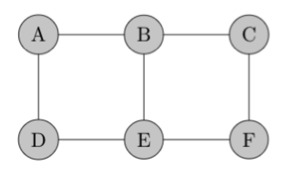
\includegraphics[width=50mm]{Figures/1.png}
    \caption{Example grid graph.}
\end{figure}

\noindent
The order of nodes, added in BFS ordering staring from A is: A, B, D, C, E, F.
Or more clearly, as presented in the figure below.
\begin{figure}[ht!]
    \centering
    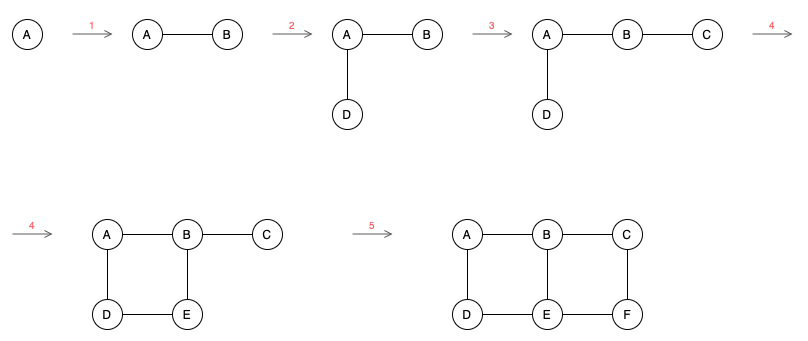
\includegraphics[width=170mm]{Figures/1_1.png}
    \caption{The order of adding nodes in BFS.}
\end{figure}

\noindent
The edge level predictions for each node, respectively as steps in BFS ordering (steps 1-5 in the figure):
\begin{itemize}
    \item 1: $S_B^{\pi} = [1]$
    \item 2: $S_D^{\pi} = [1, 0]$
    \item 3: $S_C^{\pi} = [0, 1, 0]$
    \item 4: $S_E^{\pi} = [0, 1, 1, 0]$
    \item 5: $S_F^{\pi} = [0, 0, 0, 1, 1]$
\end{itemize}
However, for $S_E^{\pi}$ and $S_F^{\pi}$, it would be enough to predict only the edges between the last three added nodes, since the shortest-path between two the farthest nodes is of distance three (following Corollary 1 from attached GraphRNN paper).
Therefore, we could write $S_E^{\pi} = [1, 1, 0]$ and $S_F^{\pi} = [0, 1, 1]$.

%%%%%%%%%%%%%%%%%%%%%%%%%%%%%%%%%%%%%%%%%%%%%%%%%%%%%%%%%%%%%%%%%%%%%%%%%%%%%%%%%%%%%%

\subsection{}

\noindent
Two advantages of graph generation using BFS ordering of nodes, as apposed to generating with a random ordering of nodes in the graph are:
\\
\textit{Less options for node orderings.} 
The number of all possible node permutations is $n!$, which is also the worst case for BFS ordering (star graphs), however, the number of observed BFS ordering on many real-world graphs is a lot smaller.
\\
\textit{Less edge predictions.} As seen in the example above when following Corollary 1, when added a new node, only last $M$ steps are enought to make edge predictions (last 3 steps in the example).
Therefore, we have only $M$ possible edges on every step, thus time complexity is $\mathcal{O}(M n)$, where $n$ is the number of added nodes, instead of $\mathcal{O}(n ^ 2)$ when checking "every node with every node".

%%%%%%%%%%%%%%%%%%%%%%%%%%%%%%%%%%%%%%%%%%%%%%%%%%%%%%%%%%%%%%%%%%%%%%%%%%%%%%%%%%%%%%
%%%%%%%%%%%%%%%%%%%%%%%%%%%%%%%%%%%%%%%%%%%%%%%%%%%%%%%%%%%%%%%%%%%%%%%%%%%%%%%%%%%%%%

\section{Subgraphs and Order Embeddings}

%%%%%%%%%%%%%%%%%%%%%%%%%%%%%%%%%%%%%%%%%%%%%%%%%%%%%%%%%%%%%%%%%%%%%%%%%%%%%%%%%%%%%%

\subsection{Transitivity}
Graph A is a subgraph of graph B and B is a subgraph of graph C, we then prove that A is a subgraph of C.
\\
Following the subgraph isomorphism definition:
\begin{align*}
    \exists \ \text{bijective} \ f : V_A \to U_B \subseteq V_B \ \text{and subgraph of B induced by } \{ f(v) | v \in V_A \} \text{ is graph-isomorphic to A.}
    \\
    \exists \ \text{bijective} \ g : V_B \to U_C \subseteq V_C \ \text{and subgraph of C induced by } \{ g(v) | v \in V_B \} \text{ is graph-isomorphic to B.}
\end{align*}
Therefore, we need to find a bijective mapping, denote it by $h$, such that $h: V_A \to U_C \subseteq V_C$ and prove that subgraph of C induced by $\{ h(v) | v \in V_A \}$ is graph-isomorphic to A.
\\
A bijective mapping $h$ could, clearly, be a compositum of mappings $g$ and $f$,
\begin{align*} 
    h = g \circ f : V_A \to U_C \subseteq V_C
\end{align*}
Assume that $a_1$ and $a_2$ are two nodes from graph A, so $a_1, a_2 \in V_A$.
Since
\begin{align*}
    f(a_1) = b_1 \in U_B \subseteq V_B
    \\
    f(a_2) = b_2 \in U_B \subseteq V_B
    \\
    g(b_1) = c_1 \in U_C \subseteq V_C 
    \\
    g(b_2) = c_2 \in U_C \subseteq V_C 
\end{align*}
using the mapping $h$ on $a_1$ and $a_2$ will give 
$$h(a_1) = g(f(a_1)) = c_1 \in U_C \subseteq V_C$$
and
$$h(a_2) = g(f(a_2)) = c_2 \in U_C \subseteq V_C$$
Thus, $ \forall a_1, a_2 \in V_A : a_1 \sim_A a_2 \Leftrightarrow  h(a_1) \sim_C h(a_2)$, so $h = (g \circ f)$ is isomorphism and A is a subgraph of C.


%%%%%%%%%%%%%%%%%%%%%%%%%%%%%%%%%%%%%%%%%%%%%%%%%%%%%%%%%%%%%%%%%%%%%%%%%%%%%%%%%%%%%%

\subsection{Anti-symmetry}
Graph A is a subgraph of graph B, and graph B is subgraph of graph A. Prove that A and B are graph-isomorphic.
\\
From $|V_A| \leq |V_B|$ and $|V_B| \leq |V_A|$ it follows that $|V_A| = |V_B|$,
so we can rewrite the subgraph isomorphic definition as
\begin{align*}
    \exists \ \text{bijective} \ f : V_A \to V_B 
    \\
    \exists \ \text{bijective} \ g : V_B \to V_A 
\end{align*}
since 
subgraph of B induced by $\{ f(v) | v \in V_A \}$ 
and subgraph of A induced by $\{ g(v) | v \in V_B \}$ in this case equals B and A, respectively.
In other words, mappings between all nodes from A and all nodes from B and vice versa are bijective.
\\
Therefore, by the definition, we can conclude that graphs A and B are isomorphic.

%%%%%%%%%%%%%%%%%%%%%%%%%%%%%%%%%%%%%%%%%%%%%%%%%%%%%%%%%%%%%%%%%%%%%%%%%%%%%%%%%%%%%%

\subsection{Common subgraph}
Prove that graph X is a common subgraph of A and B if and only if $z_x \preceq \min \{ z_A, z_B \}$, where min denotes the element-wise minimum of the two embedding vector.
\\
The proof goes in both ways (equivalence).
\\
Firstly, we assume that X is a common subgraph of A and B.
\\
For X to be a subgraph of A, the following must be true:
\begin{align*} 
    z_x \preceq z_A
\end{align*}
And similar for X to be a subgraph of B:
\begin{align*} 
    z_x \preceq z_B
\end{align*}
To make the presentation of the two possibilities easier, let us take a look at the figure below, presenting both cases.

\begin{figure}[ht!]
    \centering
    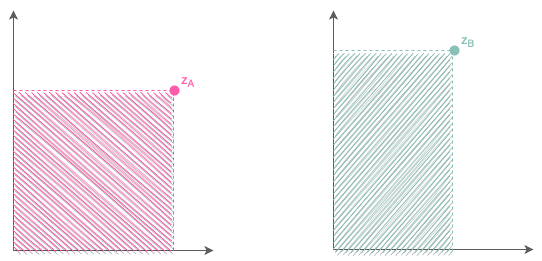
\includegraphics[width = 115mm]{Figures/2_3_a.png}
    \caption{Embedding of X must lie in the colored areas for X to be a subgraph of A in the left and B on the right graph.}
\end{figure}
\noindent
For X to be a subgraph of both, we join the two conditions, so 
\begin{align*} 
    z_x &\preceq z_A \ \text{ and } \ z_x \preceq z_B\
    \\
    \Rightarrow z_x &\preceq \min \{ z_A, z_B \}
\end{align*}

\begin{figure}[ht!]
    \centering
    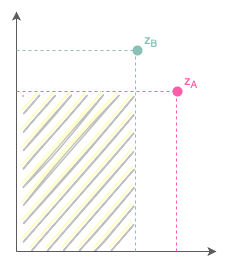
\includegraphics[width = 65mm]{Figures/2_3_b.png}
    \caption{Embedding of X must lie in the colored area for X to be a subgraph of both A and B.}
    \label{pic:emb}
\end{figure}
\noindent
Secondly, we assume $z_x \preceq \min \{ z_A, z_B \}$.
The condition is presented on the Figure \ref{pic:emb}. If the embedding of X lies in the colored area, the graph is clearly a subgraph of both A and B.
  

%%%%%%%%%%%%%%%%%%%%%%%%%%%%%%%%%%%%%%%%%%%%%%%%%%%%%%%%%%%%%%%%%%%%%%%%%%%%%%%%%%%%%%

\subsection{Order embeddings for graphs that are not subgraphs of each other}
We have the graphs A, B, C that are not subgraphs of each other. We embed them into 2-dimensional space and the condition $z_A[0] > z_B[0] > z_C[0]$ hold for first dimension.
The vizualization of the given conditions is presented in the figure below.

\begin{figure}[ht!]
    \centering
    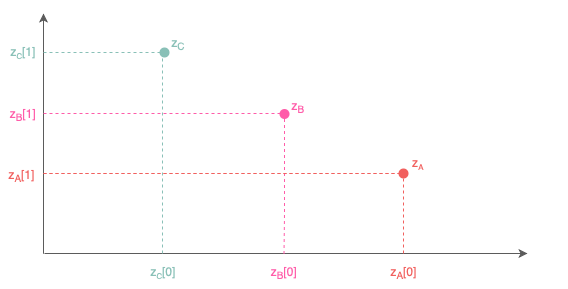
\includegraphics[width = 130mm]{Figures/2_4.png}
    \caption{Embeddings of A, B, C such that $z_A[0] > z_B[0] > z_C[0]$ hold.}
\end{figure}\label{pic:2}
\noindent
Thus, the situation presented in the figure clearly implies $z_A[1] < z_B[1] < z_C[1]$.

%%%%%%%%%%%%%%%%%%%%%%%%%%%%%%%%%%%%%%%%%%%%%%%%%%%%%%%%%%%%%%%%%%%%%%%%%%%%%%%%%%%%%%

\subsection{Limitation of 2-dimensional order embedding space}
Here we show that 2-dimensional order embedding space is not sufficient to perfectly model subgraph relationships.
\\
Suppose graphs A, B, C are non-isomorphic graphs that are not subgraphs of each other. Construct an example of graphs X, Y, Z such that they are each subgraphs of one or more graphs in \{A, B, C\}. Corresponding embeddings should satisfy $z_x \preceq z_Y$ and $z_X \preceq z_Z$.
\\
\\
Following the additional clarifications, such an example, so that each of the constructed graph is a supgraph of exactly two graphs in \{A, B, C\}, would be 
\begin{itemize}
    \item X is a subgraph of A and C,
    \item Y is a subgraph of A and B,
    \item Z is a subgraph of B and C.
\end{itemize}
From the subgraph relations above it is obvious that graph X is not a subgraph of Y and Z (because it is not subgraph of all three graphs in \{A, B, C\}).
Since without loss of generality we can suppose $z_A[0] > z_B[0] > z_C[0]$ (the situation is presented in the Figure \ref{pic:2}), there obviously exist such embeddings for X, Y and Z, such that conditions $z_x \preceq z_Y$ and $z_X \preceq z_Z$ hold, meaning X is a common subgraph of Y and Z.
Therefore, we really need higher dimensional embedding space to perfectly model subgraph relationships.

%%%%%%%%%%%%%%%%%%%%%%%%%%%%%%%%%%%%%%%%%%%%%%%%%%%%%%%%%%%%%%%%%%%%%%%%%%%%%%%%%%%%%%
%%%%%%%%%%%%%%%%%%%%%%%%%%%%%%%%%%%%%%%%%%%%%%%%%%%%%%%%%%%%%%%%%%%%%%%%%%%%%%%%%%%%%%

\end{document}